\documentclass{article}

\usepackage[UTF8]{ctex}
\usepackage{amsmath,amssymb}
\usepackage{geometry}
\usepackage{graphicx}

\geometry{a4paper, margin=2.5cm}

\begin{document}

% ============================================================
\section*{决策 Transformer（Decision Transformer / DT）}

\subsection*{先讲一个故事}

第 9 章的结尾留了一个岔路口：面对一份不能再交互的离线数据，CQL 和 IQL 选择给价值函数写进悲观，从而把估计安全地外推到数据之外。但 2020 年前后，另一个领域正在发生一场革命：GPT 证明，只要数据够多，「下一个 token 预测」这个纯监督目标就能学出复杂到惊人的行为。于是有人问了一个跨界的问题：\textbf{既然序列建模这么强，为什么还要 Bellman 方程？}

\textbf{错误做法 / 朴素做法}：把轨迹当成句子、把动作当成 token，训练 $P(a_t \mid s_t, \text{历史})$——这就是行为克隆（BC），第 9 章的及格线：数据是什么水平，策略就是什么水平，还失去了控制输出质量的能力。

\textbf{本章方法的做法}：把\textbf{期望回报}也写进序列。轨迹不再是 $(s, a)$ 的流，而是 $(\hat R, s, a)$ 的流——模型学习「在想要 $\hat R$ 这么多回报的条件下，该做什么动作」。评估时把 $\hat R$ 设成目标分数，像点歌一样点一个回报水平。

\textbf{本章的核心问题}：这到底是在\textbf{规划}，还是在\textbf{检索}训练数据里见过的轨迹？

\[
\boxed{P(\tau) = \prod_{t} P\!\left(a_t \,\Big|\, \hat{R}_{t-K+1:t},\; s_{t-K+1:t},\; a_{t-K:t-1}\right)}
\]

\subsection*{数学形式化}

一条轨迹被序列化为回报—状态—动作的交替流：

\[
\tau = \left(\hat{R}_1, s_1, a_1,\; \hat{R}_2, s_2, a_2,\; \ldots,\; \hat{R}_T, s_T, a_T\right)
\]

其中 $\hat{R}_t$ 是\textbf{return-to-go（RTG，剩余回报）}：从第 $t$ 步到回合结束的奖励总和

\[
\hat{R}_t = \sum_{k=t}^{T} r_k
\]

（折扣版本 $\sum_{k\ge t}\gamma^{k-t}r_k$ 同理；本章实验用 $\gamma=1$。）DT 是一个因果 Transformer：第 $t$ 个 token 编码 $(\hat{R}_t, s_t, a_{t-1})$，只允许注意过去，输出对 $a_t$ 的分布。训练是纯监督的交叉熵——没有 Bellman 方程、没有自举、没有 $\max$、没有价值函数：

\[
\mathcal{L}(\theta) = -\,\mathbb{E}_{\tau \sim \mathcal{D}}\left[\sum_t \log P_\theta\!\left(a_t \,\Big|\, \hat{R}_{t-K+1:t}, s_{t-K+1:t}, a_{t-K:t-1}\right)\right]
\]

$K$ 是上下文长度（本章取 16）。评估协议是本章的「遥控器」：第一步喂入目标 $\hat{R}_1 = \text{target}$，之后每走一步按定义递推

\[
\hat{R}_{t+1} = \hat{R}_t - r_t
\]

模型输出动作，环境返回奖励，RTG 相应扣减——整个闭环里没有一个价值估计。

% ============================================================
\section*{核心机制}

\subsection*{机制一：RTG 条件化——回报成为指令，但只在数据内有效}

RTG 把「策略的质量」变成了输入：同一个模型，$\hat R$ 给 50 是及格策略，给 450 是优秀策略。图~1 左图在混合质量数据（random 到 expert 全谱）上验证：目标 $\ge 200$ 时评估回报紧贴目标（200 $\to$ 210、300 $\to$ 286、500 $\to$ 335），低目标区间（50--100）只到 10--33 分——受 CartPole 可达回报下限（随机策略 $\approx 9$ 分）与低回报行为数据密度的双重限制。作为对照，去掉 RTG 输入训练的同一结构（即序列 BC）无论想要多少分，回报都钉在约 10 分（实测 9.5，随机水平）——\textbf{没有 RTG，回报无法指定}。

但指挥棒的范围由数据划界。图~1 右图把目标推到数据最优之外：600--1000 的目标不再带来任何提升（回报 259--339，方差陡增）——目标本身也成了一个会 OOD 的输入维度。RTG 本身也是一个输入维度——目标超出数据覆盖，条件分布就被推到了支撑集之外，与第 12、13 章奖励模型的「覆盖区」是同一个概念：\textbf{条件生成只会在见过的条件附近工作}。

\begin{figure}[!htbp]
  \centering
  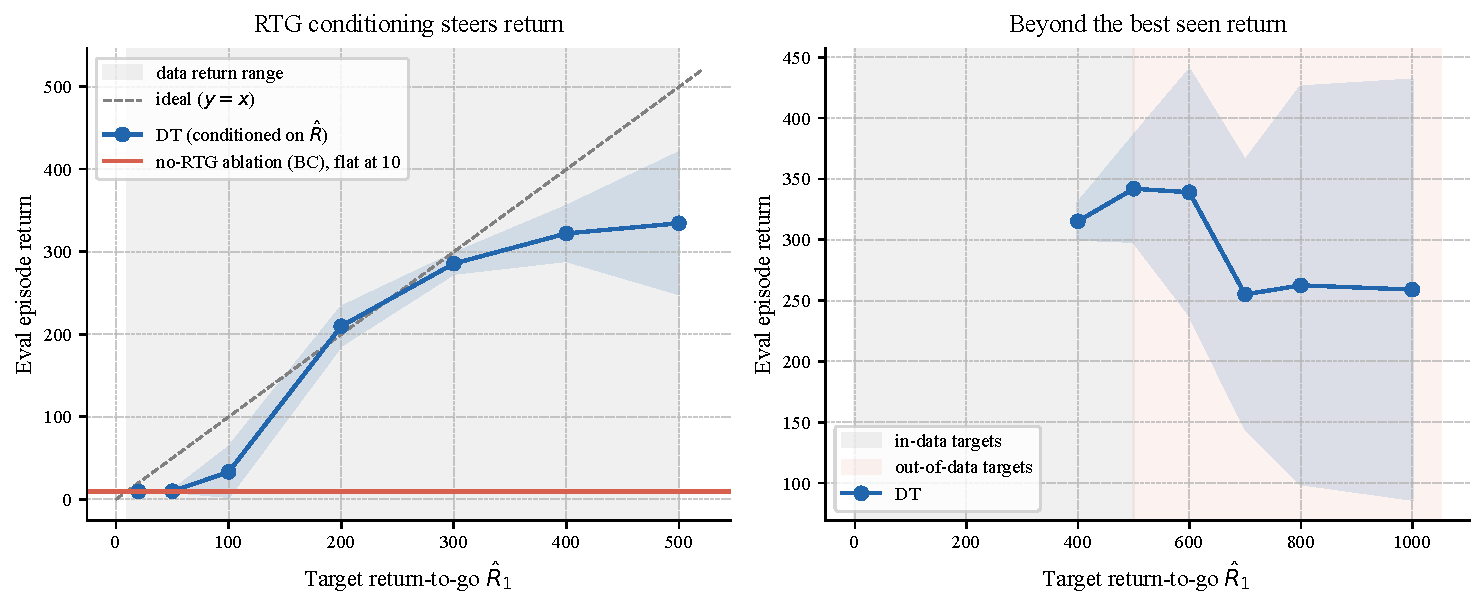
\includegraphics[width=0.98\textwidth]{fig1_rtg_conditioning.pdf}
  \caption{RTG 条件化（CartPole-v1 混合质量数据，3 个随机种子，mean $\pm$ std）。左：DT（蓝）的评估回报紧贴目标（虚线 $y=x$，灰色为数据回报范围）；无 RTG 的同结构模型（红）回报钉在固定水平——回报无法指定。右：目标超出数据最优回报后，DT 无法兑现甚至回落——条件化只在数据支撑区内有效。}
  \label{fig:dt-rtg}
\end{figure}

\subsection*{机制二：数据质量天花板——回放，不是改进}

三档数据（random / medium / expert，第 9 章同一采集配方）分别训练 DT 与 BC。图~2 的柱状对比给出一个干脆的结论：random 档数据均值 22、DT 44、BC 10；medium 档 211 / 267 / 262；expert 档 361 / 352 / 347（其中一个种子的采集策略停在 102 分，把数据均值拉低、误差条拉大——模型质量逐种子跟随数据质量）——\textbf{序列建模回放数据，不改进数据}。DT 与 BC 的差别不在能力，在可控性：DT 多了一根指挥棒，但天花板都是数据本身。

与第 9 章合起来看：CQL/IQL 用悲观化把价值外推到数据之外，medium 数据上能恢复到 BC 之上；DT 干脆不外推。这给出一条清晰的选型规则：\textbf{数据接近最优}（如演示数据、专家轨迹）时，DT 简单、稳定、还附带可控性——这正是 LLM 后训练里 SFT 的处境；\textbf{数据次优且必须超越}时，价值方法不可替代。

\begin{figure}[!htbp]
  \centering
  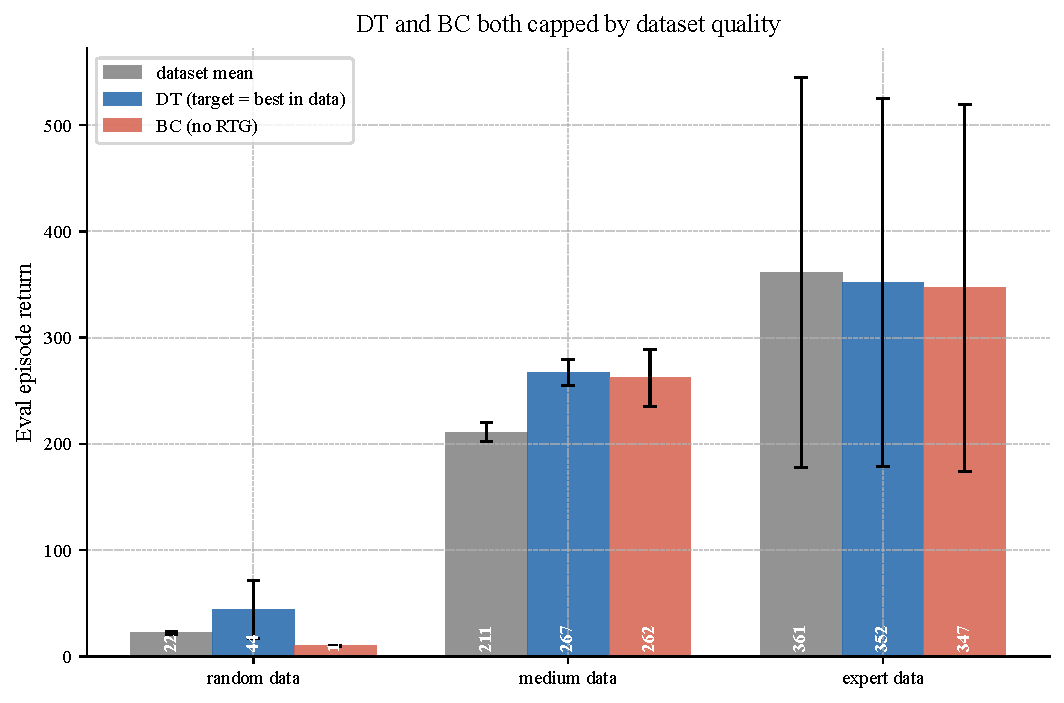
\includegraphics[width=0.88\textwidth]{fig2_data_quality.pdf}
  \caption{数据质量天花板（CartPole-v1，三档数据 × 3 个随机种子，误差条 $\pm 1\sigma$）。DT（评估目标设为数据最优回报）与 BC 的回报都贴着数据平均水平，均未超过数据质量——对比第 9 章 CQL/IQL 在 medium 数据上恢复到 BC 之上。}
  \label{fig:dt-quality}
\end{figure}

\subsection*{机制三：拼接失败——检索见过的，不组合未见过的}

「拼接（stitching）」是离线 RL 的独特能力诉求：最优轨迹的每一步转移都在数据里，只是\textbf{从未出现在同一条轨迹中}——把轨迹 A 的前半段和轨迹 B 的后半段在交汇状态处接起来，能得到数据里不存在的更优行为。第 2 章的动态规划天然会拼接：值迭代的价值像水波一样跨轨迹传播，备份不问转移来自哪条轨迹。序列建模不会：它的上下文是「一条轨迹内的历史」，模式匹配检索的是见过的整段序列。

实验把它摆到明面上（图~3）：确定性 $8\times 8$ 格子世界，最短路径 14 步；数据 400 条轨迹，最好的是 16 步——14 步路径从未整条出现，但它需要的每一步转移都在数据里。结果：表格型\textbf{离线 Q-learning 在同一份数据上拼出 14 步最优路径}；DT 条件在 $\ge 22$ 的目标上正常兑现，$\le 20$ 后进入数据稀疏区开始失效；在从未出现的 14 步目标上，90 个评估回合中有 60 个无法到达终点。

\begin{figure}[!htbp]
  \centering
  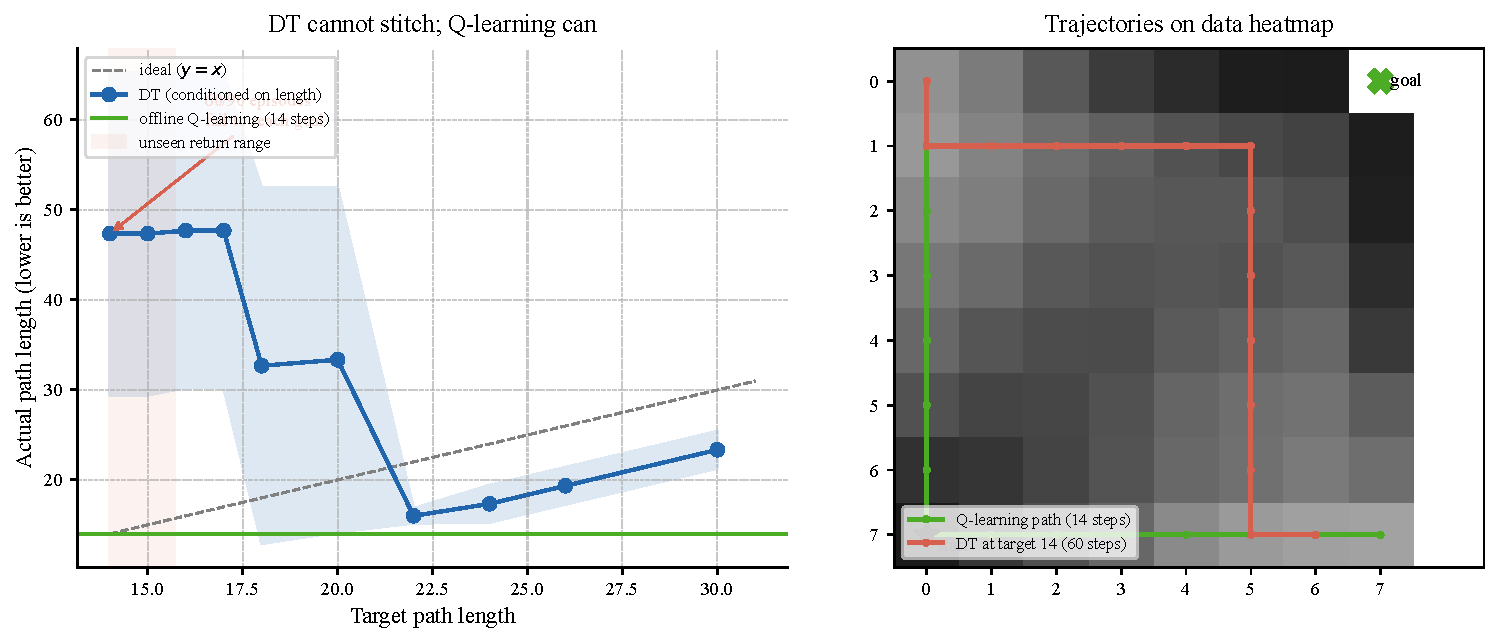
\includegraphics[width=0.98\textwidth]{fig3_stitching.pdf}
  \caption{拼接失败（确定性 $8\times 8$ 格子世界，3 个随机种子，mean $\pm$ std）。左：目标长度 $\ge$ 16（数据最优）时 DT（蓝）正常兑现；条件在最优的 14 步（红色区域，回报落到数据支撑之外）DT 失效，而离线 Q-learning（绿）在同一份数据上拼出 14 步最优路径。右：数据访问热力图与路径对比——Q-learning 的对角捷径由跨轨迹拼接而来，DT 在目标 14 下的实际轨迹偏离最优。}
  \label{fig:dt-stitch}
\end{figure}

% ============================================================
\section*{完整算法流程}

\begin{enumerate}
  \item \textbf{序列化}：把每条轨迹写成 $(\hat R_t, s_t, a_t)$ 流；状态按数据均值/方差标准化，RTG 按数据最大回报缩放；
  \item \textbf{训练}：随机采样长度 $\le K$ 的窗口（右侧对齐），最小化动作的交叉熵——纯监督，无环境交互；
  \item \textbf{评估}：初始 $\hat R_1 = \text{target}$；每步贪心（或采样）取动作，按 $\hat R_{t+1} = \hat R_t - r_t$ 递推；上下文取最近 $K$ 个 token。
\end{enumerate}

实践要点：目标回报要设在\textbf{数据范围之内}（这是与 RLHF 的 $\beta$、DPO 的训练步数并列的「隐藏超参」，设高了就是图~1 右图的 OOD 失效）；上下文长度 $K$ 权衡长程信用与训练成本；$K=1$ 时 DT 退化为最简单的条件模仿。

% ============================================================
\section*{与相邻方法对比}

\begin{center}
\begin{tabular}{c|c|c|c}
 & \textbf{BC} & \textbf{CQL / IQL} & \textbf{DT} \\
\hline
学习信号 & 监督模仿 & Bellman + 悲观 & 监督 + RTG 条件 \\
能超越数据 & 否 & 是（外推价值） & 否（回放数据） \\
能拼接 & 否 & 是（跨轨迹备份） & 否（轨迹内检索） \\
可控性（指定回报） & 无 & 无 & 有（数据范围内） \\
关键超参 & 无 & $\alpha$ / $\tau$、$\lambda$ & 目标 RTG、上下文 $K$ \\
适用场景 & 数据即目标 & 数据次优需超越 & 数据近最优 + 需要可控 \\
\end{tabular}
\end{center}

\textbf{一句话}：价值方法回答「数据之外值多少」，序列方法回答「数据之内像什么」——离线 RL 的两条哲学，谁也替代不了谁。

% ============================================================
\section*{本章在 RL 体系中的位置}

\begin{enumerate}
  \item \textbf{上游}：离线强化学习（第 9 章）给出问题与病理——分布漂移、外推误差、BC 及格线；本章换一套世界观（序列建模）重答同一道题；
  \item \underline{决策 Transformer}（本章：RL 即序列建模——回报是条件，动作是生成；三面镜子照出它的边界：条件会 OOD、数据是天花板、不会拼接）；
  \item \textbf{下游}：第 12--14 章的 RLHF、DPO、GRPO 用的语言模型与本章的 DT 是同一个物种——「序列建模 + 条件生成」是后训练一切方法的载体，差别只在条件是什么（偏好、对数比、可验证奖励）、目标从哪里来。
\end{enumerate}

读者应带走一句话：\textbf{DT 证明「序列建模」足以复现数据中的智能，也恰好只到此为止——超越数据仍然需要价值与规划}。下一章起，序列建模的这个「物种」将面对它最重要的条件输入：人类的偏好。

\subsection*{参考资料}

\begin{enumerate}
  \item Chen et al.\ (2021). Decision Transformer: Reinforcement Learning via Sequence Modeling. \textit{NeurIPS}.
  \item Janner et al.\ (2021). Offline Reinforcement Learning as One Big Sequence Modeling Problem. \textit{NeurIPS}.
  \item Brandfonbrener, Whitney \& Kakade (2022). When Does Return-Conditioned Supervised Learning Work for Offline Reinforcement Learning? \textit{NeurIPS}.
  \item Emmons et al.\ (2022). Where Did the Distribution Shift? A Causal Analysis of Behavior Cloning and Offline RL. \textit{NeurIPS}.
  \item Levine et al.\ (2020). Offline Reinforcement Learning: Tutorial, Review, and Perspectives on Practical Applications. \textit{arXiv:2005.01643}.
\end{enumerate}

\end{document}
